%*****************************************
\chapter{Data Sets}
\label{ch:datasets}
%*****************************************
This thesis deals with three different datasets: MNIST, CIFAR10, and 20Newsgroup. The associated framework contains an additional one, Reuters-21578. While the following table includes primary data about them all, the upcoming sections aim to provide a further description.
%\begin{figure}
%	\label{fig:Dataset-Attributes}
	\begin{tabularx}{\textwidth}[h]{X X X X X}
		\multicolumn{5}{X}{\textbf{Key Attributes of the Datasets}}\\
		\hline
		& MNIST & CIFAR-10 & 20-Newsgroup & Reuters-21578\\
		\hline
		\endhead
		number of datapoints & 70.000 & 60.000 & 18846  & 12.902\\
		number of labels & 10 & 10 & 20 & 10 - 115\\
		fixed split & yes & yes & "bydate" & "ModApt\'e"\\
		has metadata & no & no & yes & yes\\
		variable length & no & no & yes & yes\\
		class imbalance & no & no & no & yes\\
		multi-label & no & no & no & yes\\
	\end{tabularx}
%	\begin{tabular}{c|c|c|c|c}
%		& MNIST & CIFAR-10 & 20-Newsgroup & Reuters-21578\\
%		\hline
%		N. labels & 10 & 10 & 20 & 10 to 115\\
%		N. datapoints & 70.000 & 60.000 & 18846  & 12.902\\
%		fixed split & x & x & "bydate" & "ModApt\'e"\\
%		shortened &  &  & x & x\\
%		class imbalance &  &  &  & x\\
%		multi-label &  &  &  & x\\
%	\end{tabular}
%\end{figure}

\section{MNIST}

MNIST is a collection of gray-scale images depicting handwritten digits collected by Y. LeCun, C. Cortes, and C. J. C. Burges. The authors produced it through the recombination of SD-1 and SD-3, training set and test set of their earlier dataset NIST. They recommend MNIST as an introductory dataset for the study of image recognition methods\cite{MNIST}.\\
In 1998, Lecun et al. apply different architecture to the image classification task on MNIST, the Lenet-FCN studied in this thesis included. The simplest model, a neural network with a single dense layer, achieved 92,6 percent accuracy.\cite{lecun1998gradient}
Figure \ref{fig:MNIST-Examples} displays a few example images.
\begin{figure}
	\centering
	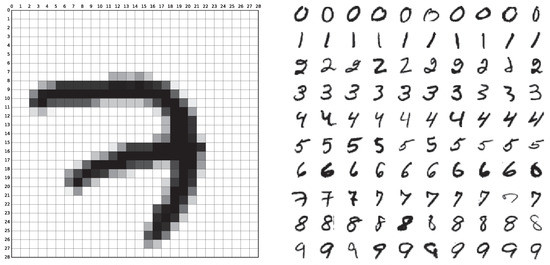
\includegraphics[width=400px]{gfx/6-Datasets/MNIST_examples_clean.jpg}
	\caption{Example images from the MNIST dataset}
	\vspace{7pt}
	\footnotesize{
		Source:\\
		https://www.mdpi.com/applsci/applsci-09-03169/article\_deploy/html/images/applsci-09-03169-g001-550.jpg
	}
	\label{fig:MNIST-Examples}
\end{figure}

\section{CIFAR-10}
CIFAR10 contains colored images of everyday objects that A. Krizhevsky, V. Nair, and G. Hinton collected out of the 80 'million tiny images' dataset. They chose datapoints with mutually exclusive labels and also provide CIFAR100, a related dataset with 100 categories. Figure \ref{fig:CIFAR10-Examples} shows 100 images from CIFAR10. \cite{CIFAR}\\
In 2014, T. Chan et al. discuss a simple deep learning network which they intend to be used as a baseline for tasks like object recognition. The architecture achieves an accuracy of 78,7 percent, more than four times the benchmark provided by A. Krizhevsky, V. Nair, and G.Hinton.\cite{CIFAR-Baseline}

\begin{figure}
	\centering
	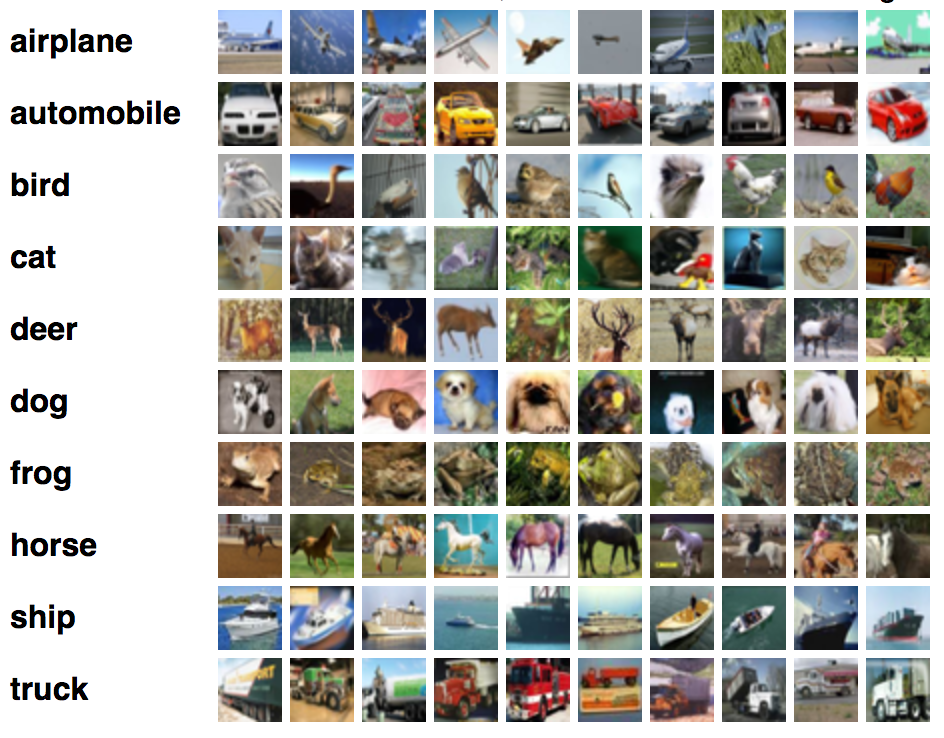
\includegraphics[width=400px]{gfx/6-Datasets/CIFAR10_examples.png}
	\caption{Example images from the CIFAR10 dataset}
	\vspace{7pt}
	\footnotesize{
		Source:\\
		https://www.cs.toronto.edu/\textasciitilde kriz/cifar.html
	}
	\label{fig:CIFAR10-Examples}
\end{figure}
\newpage

\section{20-Newsgroups}
Around 1980, a TCP-network named Usenet was established. It distributes articles\footnote{
	Transmitions obey a certain template specified by  Networks News Transfer Protocol\\
	https://tools.ietf.org/html/rfc3977
}
in a decentralized manner. Any author categorizes his articles according to a specified topic hierarchy whereafter all users of Usenet, who have subscribed to said topic, receive a copy of the document.\footnote{
	A flooding algorithm distributes the documents. Each user who receives a copy forwards it to each linked user except the original sender. Applied versions of this algorithm generally execute additional steps to avoid loops. One straightforward possibility would be to restrict any user to send each document only once
}
The text collection defined by such a topic is called a newsgroup. \cite{Usenet}\\
The dataset, 20 Newsgroups, consists of about 20.000 such articles spread over 20 topics. As Usenet defines only eight main categories, the labels in the dataset have to share some of them. The following table displays the relevant hierarchy, and figure \ref{fig:20Newsgroups-Examples} shows an example text. \cite{20-Newsgroups}

\begin{tabularx}{\textwidth}[h]{X X X}
	\multicolumn{3}{X}{\textbf{Topic of articles in 20Newsgroups}}\\
	\hline
	\endhead
	\textbf{comp.} & sys. & imb.pc.hardware\\
	& sys. & mac.hardware\\
	& os. & ms-windows.misc\\
	& windows. & x\\
	& graphics & \\
	\textbf{rec.} & sport. & baseball\\
	& sport. & hockey\\
	& autos &\\
	& motorcycles &\\
	\textbf{talk.} & politics. & misc\\
	& politics. & guns\\
	& politics. & mideast\\
	& religion. & misc\\
	\textbf{sci.} & crypt & \\
	& electronics &\\
	& med &\\
	& space &\\
	\textbf{soc.} & religion. & christian\\
	\textbf{alt.} & atheism & \\
	\textbf{misc.} & forsale & \\
\end{tabularx}

\section{Reuters-21578}
The Reuters-21578 dataset contains news articles published by the Reuters News Agency in 1987. Reuters-21578 differs from the previous data sets in the sense that it lacks a few fundamental properties. In particular Reuters-21578 is not only multi-class but rather multi-label meaning that any one data point can satisfy multiple categories. Additionally there are categories in Reuters-21578 that have no associated positive example and even for all remaining ones the amount of samples is heavily skewed. In order to restore parts of the missing properties with minimal change to the dataset different subsets of Reuters-21578 have been chosen by different researchers.\\
F. Debole \& F. Sebastiani \cite{Reuters-Subsets} describe those subsets, starting out stating that close to half of the data points are unusable which leaves 12,902 documents. 9,603 are marked for training and 3,299 for validation.\footnote{While different training-splits were used for Reuters-21578 "ModApt\'e" has become the canonical choice} They also point out the different groups of categories used for classification:
\begin{itemize}
	\item \textbf{R$\left(115\right)$}\\
	The group with the 115 categories containing at least one positive training example.\\ 
	\item \textbf{R$\left(90\right)$}\\
	The group with the 90 categories containing at least one positive training and test example.\\ 
	\item \textbf{R$\left(10\right)$}\\
	The group with the 10 categories containing the most examples. \\
\end{itemize} 


\begin{figure}
	\centering
	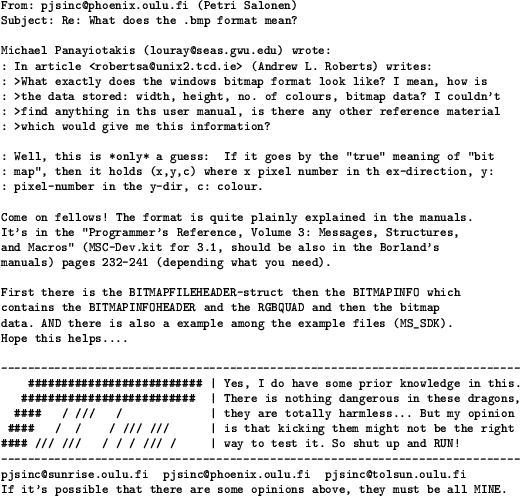
\includegraphics[width=400px]{gfx/6-Datasets/20Newsgroups_examples.png}
	\caption{An example article from the 20Newsgroups dataset}
	\vspace{7pt}
	\footnotesize{
		Source:\\
		http://strehl.com/diss/node105.html
	}
	\label{fig:20Newsgroups-Examples}
\end{figure}